% Chapter 4

\chapter{Beam Corrections} 
\captionsetup{justification=justified,singlelinecheck=false}

\label{Chapter4}

\lhead{Chapter 4. \emph{Beam Corrections}}

The parity-violating $ep$ scattering asymmetry is expected to be approximately 220~ppb at the kinematics of the \Qs experiment. The proposed goal of \Qs is to measure this asymmetry to within a few percent. This level of accuracy requires rigorous methods for distinguishing between the true parity-violating asymmetry and other sources of helicity-correlated asymmetric signals in the detectors. These false asymmetries must be measured and either removed or an error assigned to them. One of the dominant sources of false asymmetries arises from helicity-correlated beam properties. The focus of this chapter is to identify the false asymmetries arising from helicity-correlated properties of the electron beam and to explain how they are measured and removed in \Q.    

\section{Helicity-Correlated False Asymmetries}
Helicity-correlated (HC) beam properties are those properties of the electron beam whose measurement is correlated with the helicity state of the electrons. Any physical property of the electron beam other than helicity that changes with the electron helicity is a potential source of false asymmetry. As already mentioned in Section \ref{sctn:electron_source}, parity-violating experiments such as \Qs make use of a number of slow helicity reversals at different timescales in addition to the fast reversal to diagnose and remove false asymmetries. The fast reversal is accomplished using a Pockels cell to quickly reverse the source laser helicity and for \Qs the fast reversal was set at 960~Hz. A slow helicity reversal using an insertable half-wave plate (IHWP) before the Pockels cell in the source laser was used to reverse the electron helicity relative to the Pockels cell high voltage state and was changed on an 8~hour timescale. Finally, the double Wien filter was used to reverse the electron beam helicity relative to its state coming off the photo-cathode and was changed about once per month. 

Two categories of false asymmetries typically distinguished are those that cancel with IHWP reversal and those that do not. The false asymmetries that cancel with IHWP are those that have the same sign regardless of whether the IHWP is in or out of the beam, thus adding to one state and subtracting from the other and cancelling in the average. The false asymmetry that does change sign with IHWP is perhaps more subtle since it mimics the parity-violating physics asymmetry and does not cancel. False asymmetries arising from intensity asymmetries on the electron beam (beam current is systematically different between helicity states) can be readily measured and minimized. Residual intensity asymmetries are cancelled to first order by normalizing detector signals to current. False asymmetries from helicity-correlated trajectory and energy shifts on the beam depend upon individual detector sensitivities to the beam properties. Measurement of these sensitivities and correction of false asymmetries related to beam trajectory and energy constitute the subject material of the next two chapters. Further discussion of false asymmetries on the electron beam, especially those arising in the electron source, can be found in \cite{Paschke2007}.

Sensitive parity-violating experiments like \Qs employ a three-fold strategy for dealing with false asymmetries: 1) minimization, 2) cancellation and 3) correction for residual false asymmetries. The first two have to do with the experimental setup and procedure whereas the last is purely a set of analysis techniques. The main focus of this chapter is on 3, the analysis techniques used for removal of residual false asymmetries after techniques 1 and 2 have been implemented during the experiment.  
\subsection{Minimizing False Asymmetries}
Ideally, a parity-violating  experiment is set up so that false asymmetries are small relative to the physics asymmetry being measured so that additional means such as cancellation and first order corrections are effective. The following list, although not intended to be exhaustive, shows how a number of false asymmetries were minimized in both the design and operation of \Q.  
\begin{itemize}
\item {\it Alignment and azimuthal cancellation:} The \Qs experiment was designed to be azimuthally symmetric about the electron beam. The \qtor spectrometer focused elastic $ep$ scattering events onto eight quartz \v Cerenkov detector bars. Any single detector is highly sensitive to beam trajectory changes, but the average of the eight detector array cancels this sensitivity to first order due to its intrinsic azimuthal symmetry. Imagine, for example, the beam position moving to the left horizontally. The detectors on the left will experience a rate change that will be cancelled by the detectors on the right. Care was taken during the \Qs commissioning period to find the so called ``neutral axis'' of the \qtor spectrometer, that is, the beam trajectory was chosen such that the average detector sensitivity to position is minimized. Higher order effects do not necessarily cancel and any broken azimuthal symmetry such as octant to octant variations in the spectrometer field or small detector misalignments produce imperfect cancellation. 

\item {\it Source setup:} A schematic of the electron source can be seen in Figure \ref{fig:sourcetable}. High voltages across the Pockels cell used for flipping the helicity of the laser, create stresses on the crystal which can create helicity-correlated changes in the beam spot intensity, position and shape. Simply switching the direction of the high voltage across the Pockels cell does not produce exactly opposite helicity states. Furthermore, perfect circular polarization after the Pockels cell does not necessarily translate into perfect circular polarization at the cathode. Birefringent elements such as the vacuum window between the Pockels cell and the photo-cathode (see Figure \ref{fig:sourcetable}) create residual linear polarization at the photo-cathode. The strain on the GaAs crystal creates an analyzing power along the cathode strain axis for linearly polarized photons. A two-pronged approach minimizes effects from residual circulation polarization on the photo-cathode. First, a rotatable half-wave plate upstream of the vacuum window allows the axis of the residual polarization on the laser to be rotated relative to the photo-cathode analyzing axis. A prudent choice of RHWP angle will zero charge asymmetry on the beam from this effect. Second, a slightly different voltage can be set for each high voltage state of the Pockels cell. This relative small voltage offset termed a ``PITA'' (\textbf{P}olarization \textbf{I}nduced \textbf{T}ransport \textbf{A}symmetry) voltage is carefully selected to minimize charge asymmetries off the cathode. 

A series of Pockels cell position and angle scans were completed to find the optimal placement that minimizes HC deflections. Position differences on the laser are measured using a photodiode array and zeroed at the few micron level. With an ideal optical setup in the accelerator and injector, an effect called ``adiabatic damping'' reduces the beam emittance (a measure of the width of position and angle distributions in the electron beam) by a factor of $\sqrt{p_0/p}$ between the injector and the hall \cite{Paschke2007}. For the \Qs experiment with a 1.16~GeV beam and a 100~keV injector ($p_0 = 335$~keV) the position differences could be reduced in the hall by as much as a factor of 54 relative to the sourc
\item{\it Charge feedback:} During \Qs the charge asymmetry in the experimental hall was continuously monitored by a charge feedback system which adjusted the PITA voltage in real time to zero the charge asymmetry. The plot in Figure \ref{fig:charge_feedback} shows the charge asymmetry over time as the feedback system reduced the charge asymmetry.
\begin{figure}[ht]
\centering
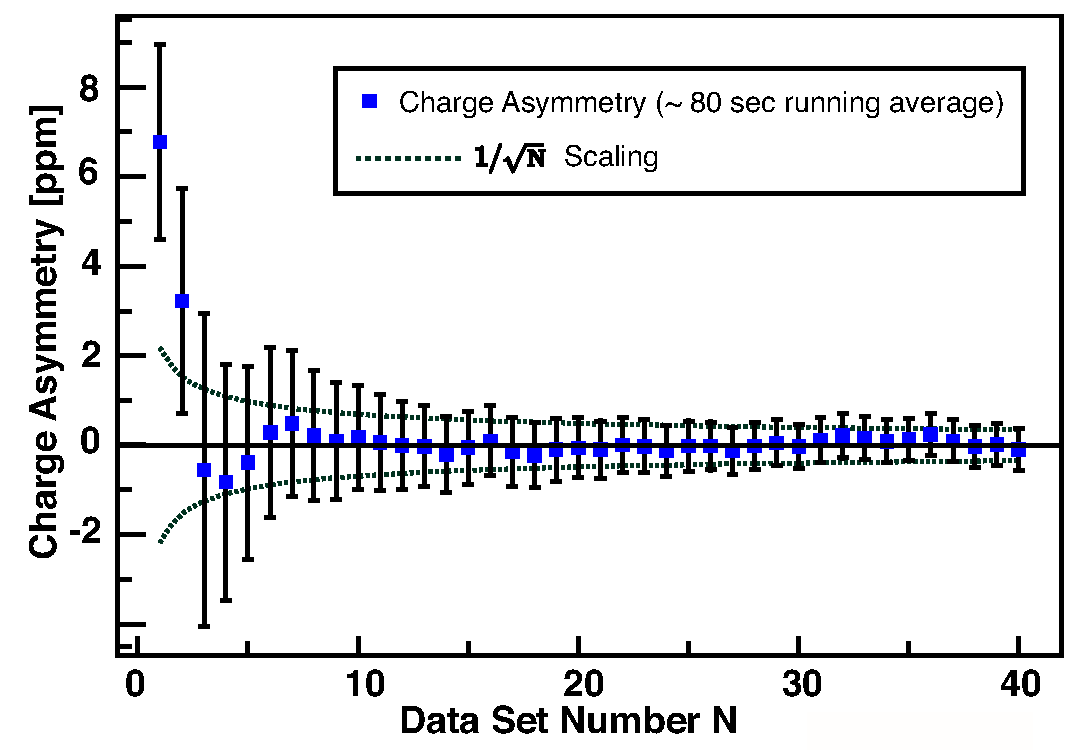
\includegraphics[width=0.7\textwidth]{Pictures/charge_feedback.pdf}
\caption{\label{fig:charge_feedback}Plot of charge asymmetry versus time over typical 1 hour run during \Qs demonstrating the action of the charge feedback system.}
\end{figure}

\item {\it Elimination of electrical pickup:} Electronics carrying the helicity signal must be isolated from the data acquisition electronics to avoid contaminating the asymmetry measurements. The source electronics which create and utilize the helicity timing signals are carefully isolated from the electronics in the experimental halls at Jefferson Lab. The helicity of the electron beam is flipped in either a $+--+$ or $-++-$ pattern, chosen to cancel linear drifts, with the sign of the first event in a quartet being determined by a pseudo-random sequence. Given the potential for contaminating the asymmetry measurement with electronics pickup from the helicity signal, \Qs utilized delayed reporting of the helicity, that is, the sign of the helicity signal sent to the data acquisition electronics was delayed by eight quartet patterns to ensure that the reported helicity was entirely uncorrelated with the actual beam helicity.

To check that no helicity-correlated signals were getting to the DAQ electronics a battery was connected to one of the channels being read out. Since the battery signal was read through the same \Qs electronics chain as the physics measurement, any asymmetry on that channel would be the signal of a false asymmetry from electronics pickup. Figure \ref{fig:battery_asym} shows the asymmetry of the battery for a typical run.
\begin{figure}[ht]
\centering
\framebox{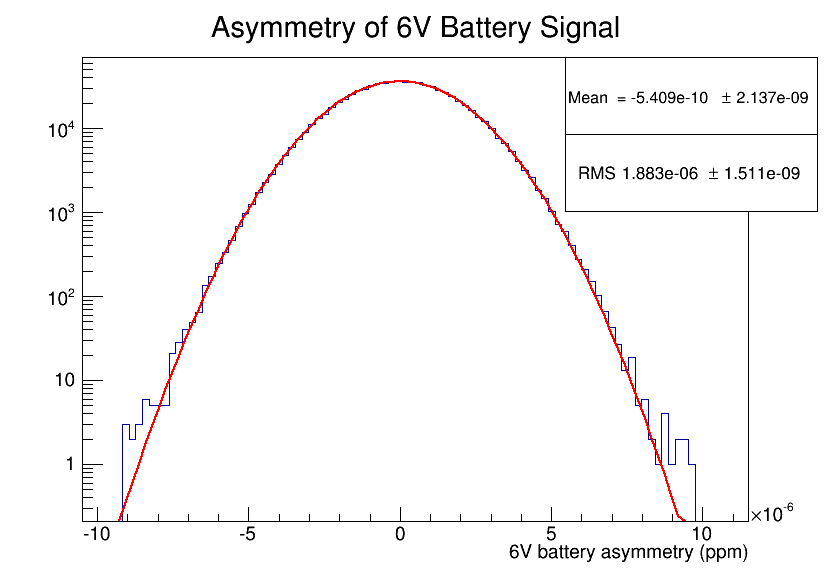
\includegraphics[width=3in]{Pictures/battery_asymmetry_run14175.png}}
\caption{Asymmetry of a 6V battery for a typical run as read out by the \Qs DAQ electronics.}
\label{fig:battery_asym}

\end{figure}

\item {\it Helicity Magnets:} For part of Run 2 the HC electron beam position differences were also suppressed by utilizing a set of helicity magnets in the injector region (see Figure \ref{fig:sourcetable}). These magnets applied a carefully calibrated helicity-correlated ``kick'' to the electron beam at the fast reversal frequency.  

\end{itemize}  
 
\subsection{Cancelling False Asymmetries}   
\Qs was designed to provide cancellation of small residual false asymmetries by the slow reversals already discussed. The pseudo-random reversal sequence cancelled helicity-correlated effects near the quartet frequency (240~Hz). The IHWP slow reversal was used to cancel effects correlated with the high voltage state of the Pockels cell. Finally, the double Wien filter was used to cancel a family of false asymmetries that flip sign with IHWP.

\subsection{Correcting for False Asymmetries}   
In principle, any property of the beam that can change rapidly with time has the potential to create a false asymmetry. For example, beam position, angle, energy, halo, polarization, intrinsic spot size, shape and intensity can all, hypothetically, create helicity-correlated false asymmetries. In practice, the four main beam properties that can be measured with sufficient speed and accuracy to make useful helicity-correlated beam correction are beam energy, position, angle and intensity. As previously mentioned, issues with beam intensity asymmetries are minimized by feedback and normalization. Two correction techniques have been applied to the \Qs data set to remove false asymmetries from HC beam trajectory and energy differences. Multivariate linear regression measures and removes detector sensitivity to beam parameters using ``beam jitter'' or variations in the parameters that naturally exist on the electron beam. ``Dithering'' or beam modulation measures the detector sensitivities with a different technique that makes use of driven beam motion, that is, intentional driven fluctuations in the beam parameters\footnote{The terms ``modulation'', ``beam modulation'' and ``dithering'' are used interchangeably throughout the text and all refer to driven beam motion. The terms ``beam jitter'', ``jitter'' and ``natural beam motion'' are also used interchangeably and refer to naturally occurring motion on the beam as opposed to driven motion.}. Due to the importance of these topics a full section will be devoted to each.

The final asymmetry reported by the \Qs experiment will be given as the straight average of the asymmetries formed from the 16 main detector PMT's. This straight average, referred to as ``PMT Average Asymmetry'' will be used in the analysis ahead where convenient. However, no PMT average ``yields'' or ``differences'' exist since both of these require intrinsic PMT-weighting (see Appendix \ref{AppendixE} for detailed definitions of these terms). Whereas linear regression operates directly on asymmetries, the beam modulation analysis measures sensitivities on detector yields. For this reason, the beam modulation analysis uses a weighted average of the main detector PMT's called MDallbars. MDallbars yields are used to calculate asymmetries which, in general, are very close to the PMT Average asymmetries. For the beam modulation analysis, the final corrections are calculated for the MDallbars asymmetries for consistency. It is important to note that final corrections calculated for MDallbars asymmetries are very close to those found for PMT Average asymmetries differing by only 0.2~ppb for Run 1 and 0.1~ppb for Run 2.  Appendix \ref{AppendixE} provides definitions of ``yield'', ``asymmetry'', ``MDallbars'' and ``PMT Average''.

%----------------------------------------------------------------------------

\section{\label{sctn:lin_reg}Linear Regression to Remove Helicity-Correlated False Asymmetries}
Linear regression utilizes the natural fluctuations in beam parameters (energy and trajectory) to determine and remove the sensitivity to these fluctuations from the data. As the name implies, any changes in the natural beam parameters are assumed to be linearly correlated to changes in the detectors. 

Linear regression in the context of \Qs is used to remove false asymmetries arising from changes in beam properties from the measured detector asymmetries. Correlations are found between detector asymmetries and helicity-correlated monitor differences, defined as the half the monitor difference between helicity states. The terminology used here is as follows: any given uncorrected detector asymmetry is $A_d$, the actual parity-violating asymmetry is $A_{PV}$, the helicity-correlated monitor differences are $\Delta X_i$ and the correction slopes are $B_i$.


Consider a model where a given detector asymmetry, $A_d$, includes the ``true'' detector parity-violating asymmetry, $A_{PV}$, that we want to measure plus other spurious signals that are linearly related to $N$ beam properties. We can express such a relationship as 
\begin{equation}
A_d=A_{PV} + \sum_{n=1}^N B_n(\Delta X_n).
\label{eq:lin_reg}
\end{equation}
Under this model, we can find the ``true'' detector asymmetry, $A_{PV}$, if we can determine the detector sensitivities, $B_n$, and the beam differences, $\Delta X_n$, as seen here:
\begin{equation}
 A_{PV}= A_d - \sum_n^k B_n(\Delta X_n).
\label{eq:lin_reg_correction}
\end{equation}
In principle, if we have $k$ orthogonal beam parameters which we can measure precisely, this is a trivial correction to make with the $B_i$ simply equal to the partial derivatives $\frac{\partial A_d}{\partial (\Delta X_i)}$. In practice, however, we are dealing with N correlated beam monitors that span the space of the $k$ orthogonal beam parameters but not equally well in all the  $k$ dimensions. In fact, some of the  $k$ parameters may not be well measured at all. For example, in the \Qs experiment, the resolution for natural beam position motion on target was much better than the resolution of natural beam angle shifts.

One method for determining the slopes $B_n$ typically used in linear regression analyses is obtained by minimizing the $\chi^2$ statistic,
\begin{equation}
\chi^2=\sum_{i}\left(\frac{(A_{d}^0)_i- \sum_n^k B_n(\Delta X_n^0)_i}{\sigma_i}\right)^2,
\label{eq:lin_reg_chi_sqare}
\end{equation} 
with respect to the slopes, $B_n$, where the sum over $i$ goes over the measured quartet asymmetries and $\sigma_i^2$ is the variance of the i'th asymmetry measurement. Here the superscript 0's indicate that all detectors and monitors have been zero-centered\footnote{ $A_d^0=A_d-\overline{A_d}$ and $\Delta X_n^0=\Delta X_n-\overline{\Delta X_n}$} since the minimization is meant only to find the best slopes to model {\bf changes} in asymmetry with {\bf changes} in monitor differences. This minimization yields
\[
\frac{\partial \chi^2}{\partial B_m}=0\Longrightarrow2\sum_{i}\left(\frac{(A_{d}^0)_i-\sum_n^k B_n(\Delta X_n^0)_i}{\sigma_i}\right)\left(\Delta X_m^0\right)=0
\]
Assuming that the variance is constant for each of the  measurements, this reduces to 
\begin{equation}
\sum_{i=1}^N(A_{d}^0)_i\left(\Delta X_m^0\right)_i=\sum_{i=1}^N\sum_{n=1}^kB_n\left(\Delta X_n^0\right)_i\left(\Delta X_m^0\right)_i.
\label{eg:lin_matrix_equation}
\end{equation}
This can be expressed in matrix form as 
\[
{\mathbf D} = \mathbf{XB},
\]
where the entries are given by
\[
D_{m}=\mathrm{Cov}[A_{d},\Delta X_m]
\]
\[
X_{m,n}=\mathrm{Cov}[\Delta X_m,\Delta X_n],
\]
and $\mathbf{B}$ is a vector of detector to monitor correction slopes. The slopes are thus given by
\begin{equation}
\mathbf{B}=\mathbf{X^{-1}D}
\label{eq:lin_reg_slopes}
\end{equation}
For the \Q~experiment, detector to beam monitor slopes were calculated from approximately 5 minutes of data taken at 240 quartets per second. A number of regression schemes were chosen using different monitor sets against which to regress the main detector. The monitor set that best measures (or spans the vector space in the language of linear algebra) the five independent beam parameters will be expected to give the most accurate results. One particular monitor set, called set 11 in the jargon of \Q, uses four target variables and beam position monitor 3c12X defined as follows:\\
\begin{itemize}
\item {targetX(Y): electron beam horizontal(vertical) position measured by extrapolating positions from beam position monitors (BPM's) in the drift region before the target downstream to the target position.}
\item {targetXSlope(YSlope): electron beam horizontal angle(vertical angle) relative to the ideal beam axis and measured by finding differences between BPM's in the drift region before the target.}
\item{BPM3c12X: the X or horizontal measurement of the BPM located in the region of highest dispersion of the electron beam in the arc leading into Hall C. BPM3c12X is highly sensitive to energy shifts and is often referred to as our ``energy monitor''.}
\end{itemize}
This particular set of BPM's is interesting because it is the same set used in the beam modulation analysis, a parallel analysis using driven beam motion to determine the correction slopes. Figures \ref{fig:Set11_X_slopes}, \ref{fig:Set11_Y_slopes}  and \ref{fig:Set11_E_slopes}  show the Set 11 regression slopes used to correct the \Qs data set. Figure  \ref{fig:Set11_E_slopes} is of particular pedagogical interest because of its tight correlation with the sensitivity of the main detector to energy. The sensitivity of the main detector to a ``true'' energy variable would be expected to be relatively stable over the course of the experiment with shifts occurring, for instance, when the current in the \qtor spectrometer or the selected beam energy were changed significantly. In the absence of these changes, energy sensitivity should be stable at the few percent level. Instead what we see is large scale shifts in main detector sensitivity to BPM3c12X, showing that this BPM is sensitive to other beam parameters as well as energy. 
The correction slope plots in figures \ref{fig:Set11_X_slopes}--\ref{fig:Set11_E_slopes} can be compared with the monitor difference plots in Appendix \ref{AppendixB} to get an idea of the full correction being applied. 


\begin{figure}[ht]
\centering

\framebox{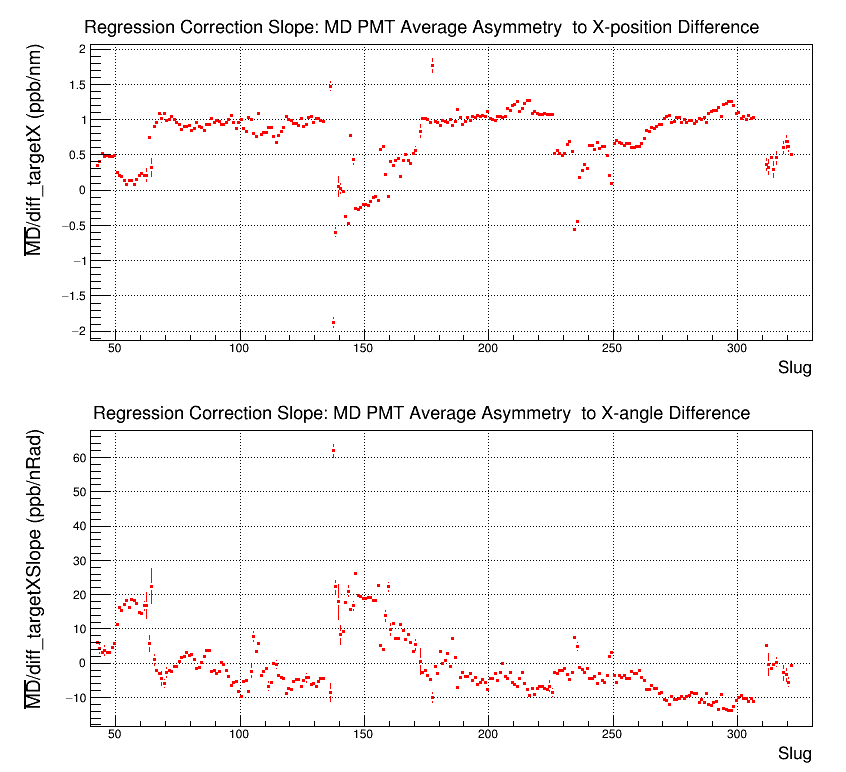
\includegraphics[width=5.5in]{Pictures/Set11_X_correction_slopes.png}}
\caption{Set 11 regression correction slopes for horizontal position and angle on target averaged over slugs ($\sim 8~hrs$).}
\label{fig:Set11_X_slopes}
\end{figure}
\begin{figure}[ht]
\centering
\framebox{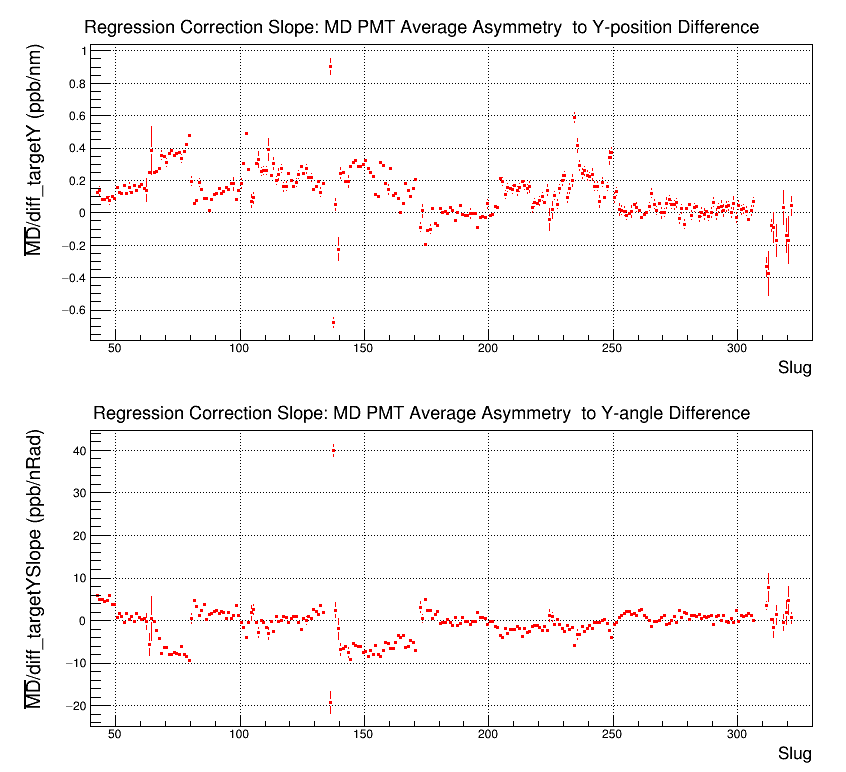
\includegraphics[width=5.5in]{Pictures/Set11_Y_correction_slopes.png}}
\caption{Set 11 regression correction slopes for vertical position and angle on target averaged over slugs ($\sim 8~hrs$).}
\label{fig:Set11_Y_slopes}
\end{figure}
\begin{figure}[h]
\centering
\framebox{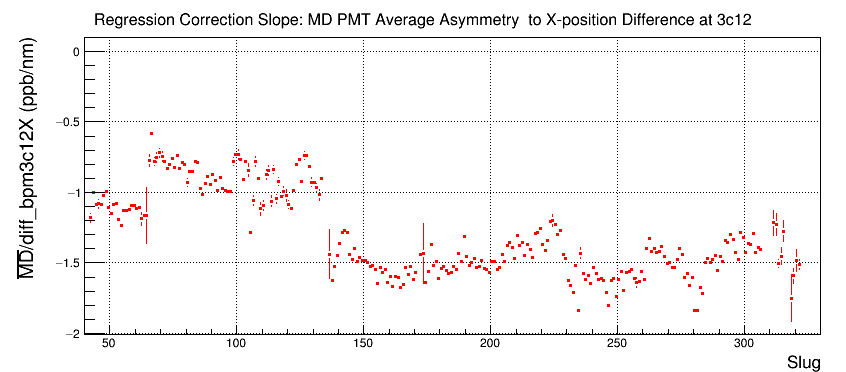
\includegraphics[width=5.5in]{Pictures/Set11_E_correction_slopes.png}}
\caption{Set 11 regression correction slopes for horizontal position at bpm3c12 averaged over slugs ($\sim 8~hrs$). This is the most energy sensitive monitor on the beamline.}
\label{fig:Set11_E_slopes}
\end{figure}
\FloatBarrier
\subsection{Bias in Multivariate Linear Regression}
In the context of the \Qs experiment linear regression minimizes noise in the detectors (dependent variables) by subtracting correlations to the beam monitors (independent variables). By definition all correlations of the detectors to monitors are removed. However, linear regression is susceptible to errors and biases. Perhaps the most glaring deficiency of linear regression arises when there is noise in the independent variables. This issue is familiar to statisticians and is called the problem of ``Errors in Variables'' (EIV). While noise in the dependent variable (detector) adds uncertainty, it does not bias the measured slope. On the other hand, noise in the independent variables (beam monitors) biases the regression correlation coefficients. In many cases where linear regression is utilized, the dependent variable is sensitive to a set of independent variables which cannot be determined accurately. Instead a measurable set of variables correlated to the set of true dependent variables is substituted. Often the substituted variables are not perfectly correlated with the true variables resulting in uncertainties and noise in the independent variables. In the case of electron scattering physics, the detectors are sensitive to beam position, angle and energy. We substitute combinations of BPM signals highly correlated to these true beam parameters. However, the BPM's introduce both correlated and uncorrelated noise which will bias the slopes.

To illustrate this point, consider a detector asymmetry $A_d$ with a sensitivity to horizontal helicity-correlated position differences in the electron beam. Regressing against position to remove the correlation using a noisy monitor $BPM$ to measure the true position differences $\Delta X$ gives 
\[
A_d=A_{PV}+\alpha\Delta X,
\]
\[
\Delta BPM = \Delta X + \delta,
\]
\[
\chi^2=\sum_{i}\left[(A_{d}^0)_i-a(\Delta BPM)_i\right]^2/\sigma_i^2
\]  
where $\delta$ is noise on the measurement of the helicity-correlated position difference $\Delta X$. Here, $\sigma_i$ is the precision on $A_d$ and $\sigma_{BPM}$ is a combination of actual beam motion (jitter) and the noise contribution from $\sigma_{\delta}$. Minimizing the $\chi^2$ statistic with respect to the desired regression slope $a$ assuming constant variance gives 
\[
a=\frac{\alpha(\sigma_{BPM}^2-\sigma_{\delta}^2)}{\sigma_{BPM}^2}=\alpha\left(1-\frac{\sigma_{\delta}^2}{\sigma_{BPM}^2}\right).
\]
This also assumes that the $\delta$ is uncorrelated with $\Delta X$ (which may or may not be true). Notice that coefficient, $a$, is diluted relative to the desired correlation coefficient, $\alpha$, to which the detector is sensitive. Statisticians refer to this effect as ``regression dilution'' or ``regression attenuation'' since the bias for a single regressor with noise is always toward zero. On the other hand, if $\delta$ and $\Delta X$ are correlated, the coefficient can be biased in either direction, although dilution is generally expected.\footnote{Economist Jerry Hausman calls this the ``Iron law of econometrics''--the magnitude of the estimate is usually smaller than expected.''\cite{Hausman}}

It is useful to point out an effect similar to this in the \Qs dataset. In order to correct for residual charge asymmetries on the electron beam, all detector measurements were normalized to the measured current. Of course, any noise in the BCM('s) used to normalize the detector will be introduced into the detector data. This added noise gives the appearance of detector sensitivity to charge when regressing against the same BCM(s) used in the normalization. Naively one might be tempted to regress against charge to remove this sensitivity. Linear regression schemes which include charge, do indeed find a residual detector to charge sensitivity and assign an additional correction. The effect of this can be easily seen in Table \ref{tab:regression_corrections_table}. The four columns show corrections assigned to the data using different monitor sets as regressors. Set 3 is the only set in the table that includes a sixth regression variable, charge. In particular, notice the variation in the corrections for the first 5 Wien states. Wien states from 6 to 10 have much less variation between the charge included and charge excluded regression schemes. One reason for this difference is bias introduced by the BCM's used in the regression scheme. For the first 5 Wien states, set 3 used BCM's 1 and 2, whereas the Wien states 6-10 used BCM's 7 and 8. BCM's 7 and 8 had new digital electronics which greatly reduced the width of their intrinsic noise by about a factor of two from the analog electronics used to read out BCM's 1 and 2 (see Figure \ref{fig:BCM_dd_width}). 


\begin{table}[h]
\caption{Corrections for regression with various monitor sets shown averaged over Wien states. All corrections are weighted by the reciprocal of the square of the main detector error. {\it Note: this table is for purposes of comparison of various regression schemes and does not contain the actual correction and asymmetry values used for \Q. It contains only the data for which there are good regression slopes for all schemes shown.} The columns represent regression schemes using different monitor sets. Standard uses the target variables (targetX(Y), targetX(Y)Slope, and energy. Set 11 uses the target variables and the most energy-sensitive monitor BPM3c12X. Set 3 is the same as Set 11 except that charge is added as a sixth regressor. For definitions of these variables see Appendix \ref{AppendixE}.}
\begin{center}
\begin{tabular}[ht]{|l|c|c|c|c|}\hline
Wien & Raw Asymmetry & Standard &~~Set11~~&~~Set3~~~\\
~ & (ppb) & (ppb) & (ppb) & (ppb) \\\hline
  1  & -337.2 & +6.5  & +6.5 & +5.5 \\\hline
  2  & -192.2 & +38.0 & +38.0 & +50.6 \\\hline
  3  & -257.2 & -25.6 & -25.6 & -25.6 \\\hline
  4  & -270.7 & -6.1  & -6.1 & -3.5 \\\hline
  5  & -191.6 & -9.5  & -9.5 & -11.3 \\\hline
  6  & -207.0 & -25.6 & -25.6 & -25.5 \\\hline
  7  & -123.6 & +33.5 & +33.5 & +33.7 \\\hline
  8a & -184.5 & -12.9 & -12.9 & -12.8 \\\hline
  8b & -157.8 & -2.4  & -2.4 & -2.4 \\\hline
  9a & -137.9 & -0.5  & +0.3 & -0.5 \\\hline
  9b & -158.1 & +1.6  & +1.6 & +1.8 \\\hline
  10 & -222.7 & -6.7  & -6.7 & -4.7 \\\hline
\end{tabular}
\end{center}
\label{tab:regression_corrections_table}
\end{table}

One evidence for bias arising from noisy monitors used in regression is a dependence of the correlations on the timescale of averaging utilized. The default method for determining regression correlations is to measure them at the quartet level, that is, at the smallest timescale for measured asymmetries in the \Qs experiment. If one chooses instead to average data over a longer period and then find the correlations between the averages, often one arrives at a different solution. One source of the difference is noise in the beam monitors that averages to zero over time. This effect can be seen in Figure \ref{fig:regression_bias} where the correlation of the MDallbars to targetX differences for the same data are determined with different averaging timescales. Although one might expect that longer averages might yield correlations closer to the desired ones, complications arise at longer timescale averaged from long term changes in beam conditions. Also, the longer average correlations have increased errors in the slopes due to decrease in the range of the independent variables and the number of data points. 
\begin{figure}
\centering
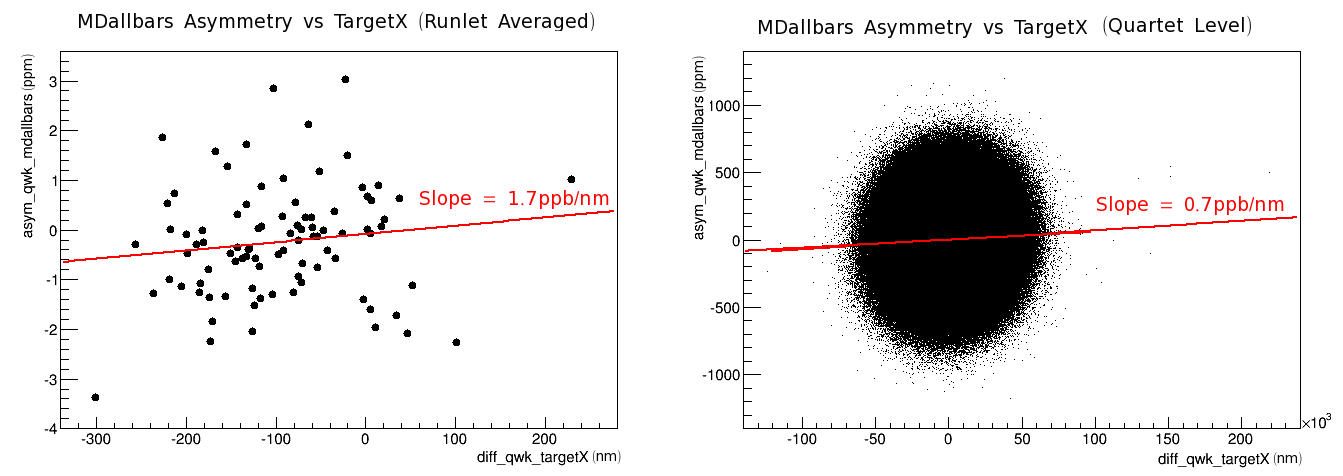
\includegraphics[width=5.8in]{./Pictures/Regression_bias_example.png}
\caption{\label{fig:regression_bias}Correlation between MDallbars asymmetry and targetX differences over a few hours during Run 2. Each point in the left plot is an average over a runlet (4-5 minutes) whereas each point in the right plot is an asymmetry measured at the quartet level (4~ms). The effect of regression dilution from noise in the position monitor is evident in the smaller measured slope for the quartet level plot.} 
\end{figure}

Another weakness in linear regression found to be an issue during \Qs concerns the use of natural beam motion. Although the beam is assumed to move in position, angle and energy, its motion may be small enough that it is below or close to the resolution of the beam monitors. When the natural motion of the beam is close to the monitor resolution limit in one or more of the parameters, those parameters will not be assigned a correct slope. In this case a ``quiet'' beam may be more difficult to correct than a noisy one. It is important to note that small differences in the beam at or near the monitor resolution limit does not mean that the detector system is not sensitive to those parameters, nor that the correction to the main detector from those parameters will be insignificant. An in depth study of the monitor sensitivities to beam motion during \Qs showed that, in fact, the differences in beam angle at the target were close to the monitor resolution level creating doubts as to the reliability of linear regression for assigning corrections for beam parameters. This study suggests that regression corrections are most reliable when the beam motion is more than 8 times the monitor resolution. The details of this study will be included in a future thesis \cite{Peng}.

Despite the weaknesses and biases inherent in the use of linear regression, it remains a useful tool. However, an independent method of determining corrections is highly desirable.


\section{Beam Modulation to Remove Helicity-Correlated False Asymmetries}
Beam modulation or beam dithering provides an alternate method to determine correction slopes for removing detector sensitivity to electron beam parameters. By deliberately modulating the five known beam parameters with some known drive signal and simultaneously measuring the detector and beam monitor responses to the modulation, it is possible to back out the requisite detector to monitor responses. Although it would be convenient to be able to modulate the beam purely in each of the five orthogonal beam parameters, in practice this is not easily accomplished. Instead five independent but not necessarily orthogonal modulations of the beam properties are used. It is helpful to think of a 5-dimensional parameter space composed of horizontal position (X) and angle (X'), vertical position (Y) and angle (Y') and energy (E). For a linear system, the five modulation types can be thought of as five independent straight line trajectories or vectors in this space. These modulation vectors are often referred to as ``coils'' since the position and angle trajectories are driven by air coil magnets. There are also five monitors whose sensitivities can be described by five independent vectors in this space. Finally, any component of the detector signal that can be described in this 5-D space must be characterized and removed. Given a set of coils $C_c$ driving the beam, the coils as well as monitor and detector responses can be expressed as
\begin{align}
Coil_c=C_c=\delta_C+\sum_{i=1}^{N}\gamma_{ic}X_i\\
Monitor_{m}=M_{mc}=\delta_M+\sum_{i=1}^{5}\alpha_{i}^{(m)}X_i\\
Detector_{d}=D_{dc}=\delta_D+\sum_{i=1}^{5}\beta_{i}^{(d)}X_i,
\label{eq:5parameter_space}
\end{align}
where the $X_i's$ are the five ideal orthogonal parameters (X,Y,X',Y',E). The coils $C_c$ are abstract quantities that refer to the effects of the modulation of magnetic coils and the RF cavity on the electron beam.\footnote{This picture of the coils, detectors and monitors as vectors in an abstract 5D space is an idea that was useful to the author but is a potential source of confusion. The idea being conveyed is that detector and monitor sensitivities ($\alpha_i,~\beta_i$) to these 5 dimensions can be thought of as vectors. The coils have the ability to move the electron beam along 5 independent straight-line trajectories in this 5D space but these trajectories are neither precisely orthogonal nor coincident with the 5 axes of this space. The coil vectors then, are inputs or forces, whereas the monitor and detector inputs are motions or responses. For example, in the \Qs setup, Coil 0 primarily moves the beam along some combination of horizontal position and angle change and might be represented as vector (a,0,b,0,0). The modulation analysis simply determines the dot products of the monitor and detector response vectors with the coil vectors by measuring the responses to the coils $\frac{\partial D_{dc}}{\partial C_c}$ and $\frac{\partial M_{mc}}{\partial C_c}$. For example, the detector response to coil $C_c$ is given by \[\frac{\partial D_{dc}}{\partial C_c}={\bf D_{d}\cdot C_c}=(\beta_{1},\beta_{2},\beta_{3},\beta_{4},\beta_{5})\cdot(\gamma_{0c},\gamma_{1c},\gamma_{2c},\gamma_{3c},\gamma_{4c})=\sum_{i=1}^5\beta_{ic}\gamma_{ic},\] where the detector response $\frac{\partial D_{dc}}{\partial C_c}$ is measured and the $\beta$'s and $\gamma's$ are not determined. It will be shown that as long the monitor set and coil set are chosen such that both span the 5D space, these detector and monitor responses to the five coils are sufficient to fully determine corrections to the five beam parameters. Knowledge of the composition of the coils, monitors and detectors in the ideal orthogonal basis is not required. } $M_{m}$ and $D_{d}$, on the other hand, are monitor and detector signals which include responses to beam parameters. The monitor and detector sensitivities to beam motion in the five dimensions are the $\alpha_i$'s and $\beta_i$'s respectively. The $\delta_C$ is a component of the modulation not well described by the five parameters and is expected to be 0 on average with noise that is small compared to the driven motion. A non-zero $\delta_C$ would mean that the coils are modulating the beam in a mode not described by the five expected parameters X, X', Y, Y' and E ({\it eg.} beam spot size). The $\delta_M$ term is a component of the monitor signal not described by the 5 parameters and may be attributed to effects such as electronics noise or resolution error. Finally, the $\delta_D$ term is the part of the detector signal which is insensitive to motion in the five beam parameters. The parity-violating asymmetry is part of the $\delta_D$ term. Here the detectors and monitors are actual measured yields not helicity-correlated differences as in the linear regression analysis. $M$ is the monitor reading and $D$ is the detector signal both averaged over an MPS window.  Rearranging the detector equation in \ref{eq:5parameter_space} gives
\[
\delta_D = D_d-\sum_{i=1}^{5}\beta_iX_i.
\]  
Taking the differential of the monitors and detectors with respect to the coils removes the independent $\delta$ terms giving
\begin{eqnarray}
\frac{\partial M_m}{\partial C_c}=\sum_{i=1}^{5}\frac{\partial M_m}{\partial X_i}\frac{\partial X_i}{\partial C_c}\\
\frac{\partial D_d}{\partial C_c}=\sum_{i=1}^{5}\frac{\partial D_d}{\partial X_i}\frac{\partial X_i}{\partial C_c}
\label{eq:5parameter_differential}
\end{eqnarray}
Now inserting an identity operator allows us to express Equation \ref{eq:5parameter_differential} as
\begin{equation}
\frac{\partial D_d}{\partial C_c}=\sum_{i=1}^{5}\frac{\partial D_d}{\partial X_i}\left(\frac{1}{5}\sum_{m=1}^5\frac{\partial X_i}{\partial M_m}\frac{\partial M_m}{\partial X_i}\right)\frac{\partial X_i}{\partial C_c}=\sum_{m=1}^{5}\frac{\partial D_d}{\partial M_m}\frac{\partial M_m}{\partial C_c},
\label{eq:det_to_coil}
\end{equation}
which we recognize as a simple change of basis from the five ideal, orthogonal parameters to our set of five monitors. This can be expressed as a matrix equation
\[
\mathbf{A=R\cdot S},
\]
where $\mathbf A$ is the vector of detector to coil sensitivities, $\mathbf R$ is the matrix of monitor to coil sensitivities and  $\mathbf S$ is the vector of detector-to-monitor correction slopes which can be solved for ${\bf S=R^-1A}$. 

Equation \ref{eq:det_to_coil} represents an exact solution assuming no error in the measured responses which is, of course, never the case. However, if the beam is driven in more than five ways, that is, if more than 5 coils are utilized, this extra information can be used to reduce the error in the solution, provided all coils yield constistent information about the beam/monitor/detector responses. One could imagine, for example, driving the beam with pure horizontal motion and then pure vertical motion and then along a straight line at 45$^{\circ}$. The extra driving mode (coil) should reduce noise in the solution but not give additional information. If N coils or driving modes are used, one ends up with N equations in 5 unknowns (5 correction slopes $\frac{\partial D_d}{\partial M_k}$). The best solution to this set of equations can be found by minimizing the $\chi ^2$ statistic independently for each detector $D_d$
\begin{equation}
\chi^2=\sum_{i=1}^N\left(\frac{\partial D_d}{\partial C_i} - \sum_{m=1}^{5}\frac{\partial D_d}{\partial M_m}\frac{\partial M_m}{\partial C_i} \right)^2/\sigma_i^2,
\label{eq:chisquare}
\end{equation}

where the sum is over N coils. Note that since the beam is still assumed to have five degrees of freedom, five monitors are still used. Taking the derivative with respect to the detector slopes, $\frac{\partial D_d}{\partial M_k}$, and setting the equation equal to 0 gives
\[
\frac{\partial\chi^2}{\partial\left( \frac{\partial D_d}{\partial M_m}\right)}=-2\sum_{i=0}^N\frac{1}{\sigma_i^2}\left(\frac{\partial D_d}{\partial C_i}- \sum_{m=1}^{5}\frac{\partial D_d}{\partial M_m}\frac{\partial M_m}{\partial C_i} \right)\frac{\partial M_m}{\partial C_i} = 0.
\]
If we assume that the detector noise is constant over all coil measurements,that is, that all responses are equally well determined the solution is given by
\footnote{Under the approximation of equal variance this procedure is the same as finding the Moore-Penrose matrix inverse often called the ``generalized inverse'' or ``pseudoinverse'' (see for example http://mathworld.wolfram.com/Moore-PenroseMatrixInverse.html), which is the ``shortest length least squares solution to'' ${\bf b=Mx}$. Multiplying both sides by ${\bf M^T}$ gives  ${\bf M^Tb=M^TMx}$ which is the same as Equation \ref{eq:chisquaresolution_no_variance}, with a solution  ${\bf x=(M^TM)^{-1}Mb}$. {$\bf M^+=(M^TM)^{-1}M$} is the definition of the Moore-Penrose matrix inverse for pure real matrices.}
\begin{equation}
\sum_{i=1}^N\left(\frac{\partial D_d}{\partial C_i}\frac{\partial M_k}{\partial C_i}\right) = \sum_{m=1}^5\frac{\partial D_d}{\partial M_m}\sum_{i=1}^N\left(\frac{\partial M_m}{\partial C_i}\frac{\partial M_k}{\partial C_i} \right). 
\label{eq:chisquaresolution_no_variance}
\end{equation}
Explicitly writing this for the set of five monitors and a single detector index yields
\[
\mathbf{R^TA=R^TR\cdot S}\longrightarrow\mathbf{B=M\cdot S},
\]
where ${\bf B=R^TA}$ and ${\bf M=R^TR}$ is a square symmetric matrix. Here ${\bf A, S}$ and ${\bf R}$ defined the same as in Equation \ref{eq:det_to_coil}.
\begin{equation}
\left(\begin{array}{c}\sum_i\frac{\partial D_d}{\partial C_i}\frac{\partial M_1}{\partial C_i}\\\sum_i\frac{\partial D_d}{\partial C_i}\frac{\partial M_2}{\partial C_i}\\\sum_i\frac{\partial D_d}{\partial C_i}\frac{\partial M_3}{\partial C_i}\\\sum_i\frac{\partial D_d}{\partial C_i}\frac{\partial M_4}{\partial C_i}\\\sum_i\frac{\partial D_d}{\partial C_i}\frac{\partial M_5}{\partial C_i}\end{array}\right)=\left(\begin{array}{ccccc} M_{11} & M_{12} & M_{13} & M_{14} & M_{15}\\ M_{21} & M_{22} & M_{23} & M_{24} & M_{25}\\M_{31} & M_{32} & M_{33} & M_{34} & M_{35}\\M_{41} & M_{42} & M_{43} & M_{44} & M_{45}\\M_{51} & M_{52} & M_{53} & M_{54} & M_{55}\end{array}\right) \left(\begin{array}{c}\frac{\partial D_d}{\partial M_1}\\\frac{\partial D_d}{\partial M_2}\\\frac{\partial D_d}{\partial M_3}\\\frac{\partial D_d}{\partial M_4}\\\frac{\partial D_d}{\partial M_5}\\\end{array}\right),
\label{eq:chisquare_matrix}
\end{equation}
where 
\[
M_{jk}=\sum_{i=1}^N\left(\frac{\partial M_j}{\partial C_i}\frac{\partial M_k}{\partial C_i}\right).
\]
The correction slopes are then given by 
\begin{equation}
\mathbf{S=M^{-1}\cdot B}.
\label{eq:solution_to_matrix}
\end{equation}

At this point it is helpful to point out the fundamental differences between linear regression and beam modulation for determining correction slopes. First, because the beam modulation analysis re-expresses detector and monitor sensitivities in the 5-parameter coil basis (which is designed to be over position, angle and energy) any correlations that exist outside this five parameter space will not be removed. Second, because all correlations are measured relative to a well-determined variable, that is, the phase of the coil being modulated, the issue of ``noise in independent variables'' or ``noise in regressors'' which creates biases in linear regression, is almost non-existent for the beam modulation analysis. Noise in the monitors will not bias the calculated slopes in the modulation analysis unless the noise happens to be at the precise frequency of the drive signal. Also, in practice, driven motion is much larger than natural motion so that measurement of the beam motion is not limited by the monitor resolution. Third, when beam modulation fails to find the proper correction slopes, its failure can be evidenced in residual sensitivity to the modulation coils if the system is over-determined\footnote{In this context over-determined means the system is driven by more modulation coils than there are expected degrees of freedom. For \Qs there were a total of 9 modulation modes used for only 5 expected degrees of freedom on the electron beam.}. Success in nulling sensitivity to the coils is not guaranteed by design unless the number of coils used in the analysis is equal to the number of degrees of freedom. Linear regression, on the other hand, is guaranteed by design to null first order correlations to the monitors at the sampling frequency. This is not to say that the failure of the modulation technique to give the proper slopes must be evident in residual sensitivity. There are subtle ways for the modulation analysis to fail without leaving residual sensitivity to the coils. The failure modes of the modulation analysis will be discussed in a future section. 

\subsection{Fast Feedback and Beam Modulation}
The beam modulation system, introduced in Chapter 3, was designed with a pair of air core dipole magnets to drive vertical motion and another pair for horizontal motion.  Sinusoidal waveforms created by function generators were sent to the modulation coils to drive the motion. The amplitudes of the waveforms sent to the  modulation coils were chosen to create four independent trajectory-related motions at the target position. Modulation of energy, the fifth degree of freedom, was accomplished via a sinusoidal waveform sent to a Vernier on an accelerating RF cavity in the south linac. Further details on the studies and models that went into the design, position and choice of waveform amplitudes can be found in \cite{Nur}.

The electron beam at Jefferson Lab has natural position and angle noise, termed ``beam jitter''. A Fast Feedback (FFB) system was designed to produce trajectory and energy shifts to cancel natural beam jitter at the target. The FFB system was designed particularly to remove low frequency motion of the beam ($<$80~Hz) as well as the first few harmonics of 60~Hz line noise \cite{Lebedev}. Like the beam modulation system, it utilizes air core dipole magnets and Verniers on RF accelerating cavities to manipulate the beam trajectory and energy. In principle, if the FFB system is operating properly during beam modulation it should null the effects of the modulation coils at the target by removing sensitivity to the modulation frequency. However, for the majority of the Qweak experiment, FFB was found to be ineffective at nulling driven beam position and angle motion at the target. As a result, the decision was made to leave FFB engaged during periods of position and angle modulation. The FFB system was paused during energy modulation because it was found to be very effective at nulling the beam energy shifts. Looking at Figures \ref{fig:bpm_amplitude_vs_z_xmod} and \ref{fig:bpm_amplitude_vs_z_ymod} we can see the response of the beam to the four different types of trajectory modulation both with FFB on and off as a function of distance along the beamline upstream from the target. Since the FFB on and off data shown were taken about 3 weeks apart some of the differences may be attributed to optics changes on the beamline; however, the plots clearly show that even with FFB on, the modulation system successfully drives large amplitude excursions at the target.
\begin{figure}[ht]
\centering
\framebox{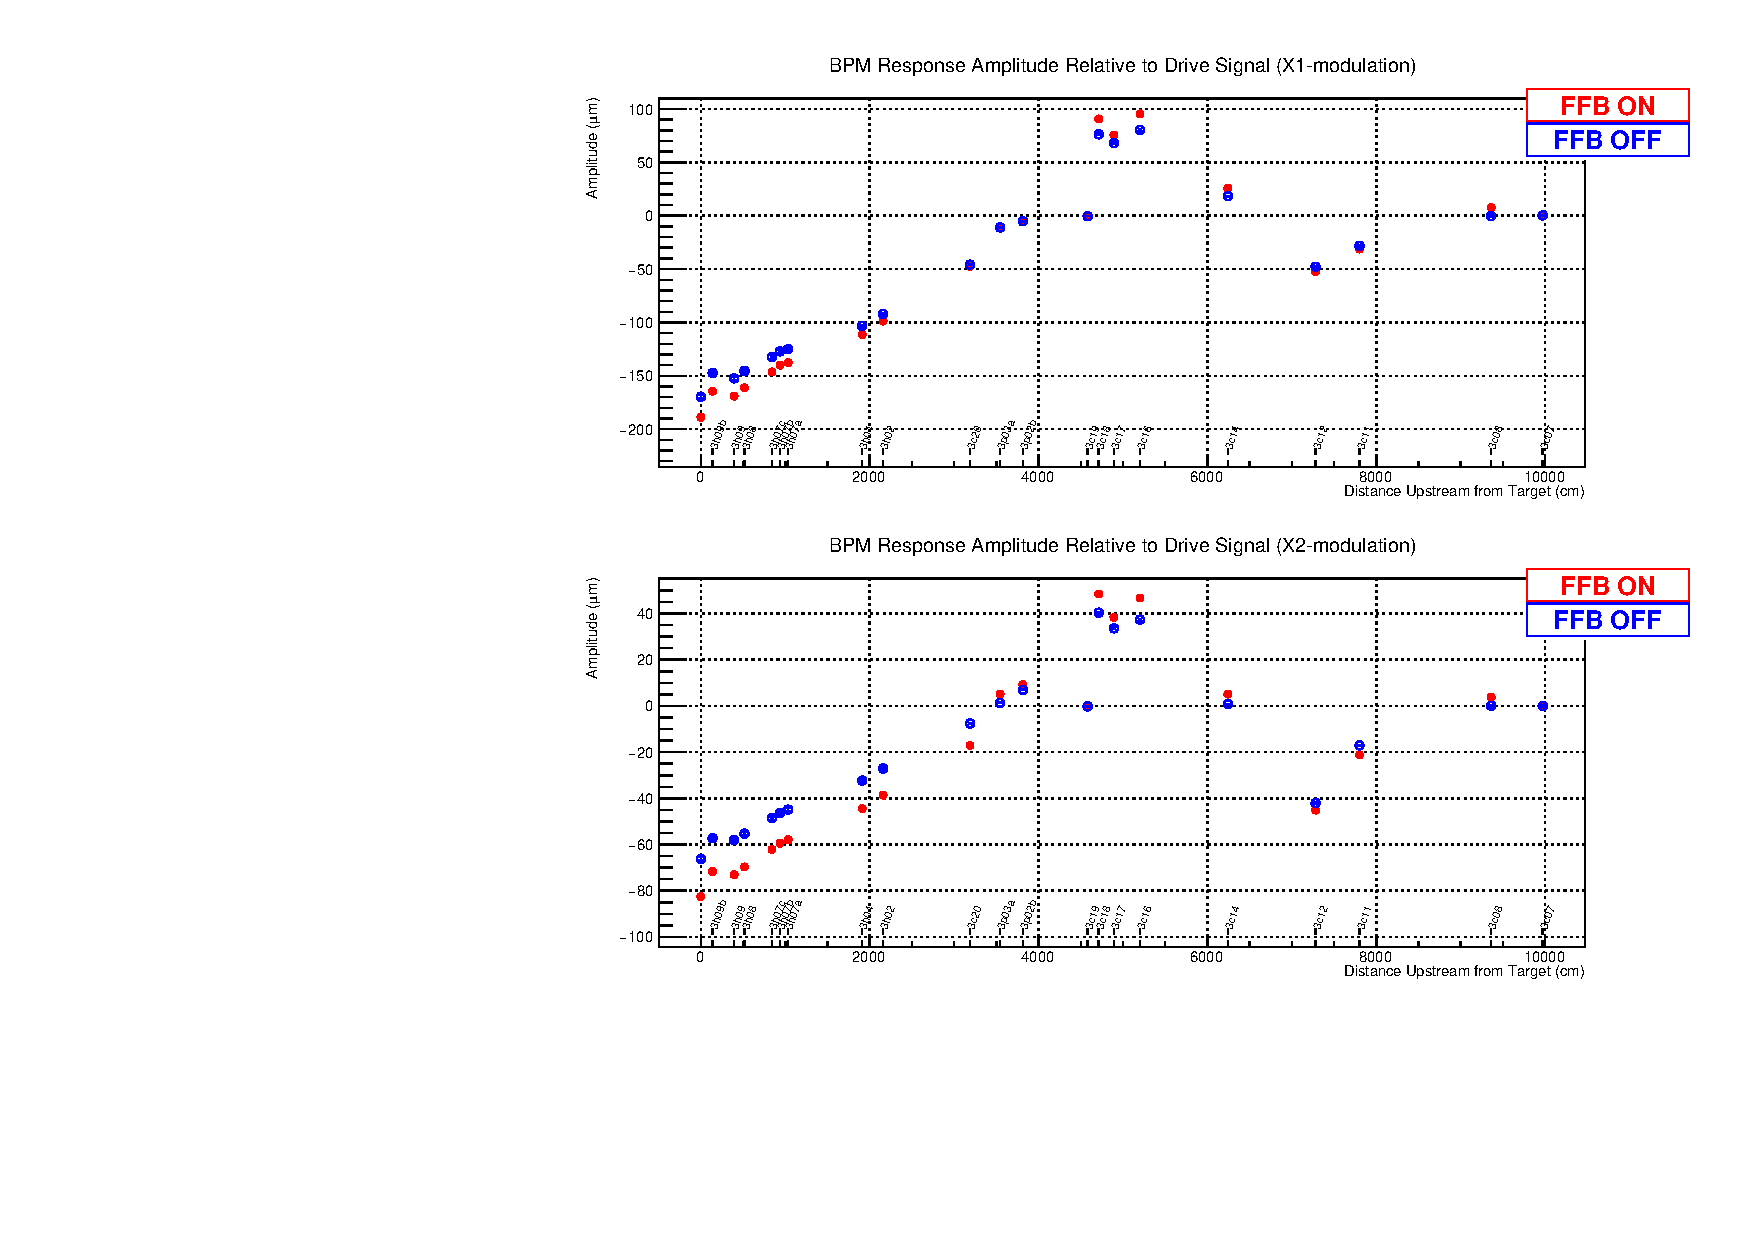
\includegraphics[width=5.6in]{Pictures/bpm_amplitude_vs_z_xmod.pdf}}
\caption{Amplitude of BPM response as a function of distance along beamline upstream from the target. Shown is X-response to two types of horizontal modulation. Notice the relatively small difference between FFB on and FFB off. This data corresponds to $A(z,\phi)$ in Equation \ref{eq:z_dep_response}. The data for FFB off came from 18445 and for FFB on from 17445 taken about 3 weeks apart.}
\label{fig:bpm_amplitude_vs_z_xmod}
\end{figure}
\begin{figure}[ht]
\centering
\framebox{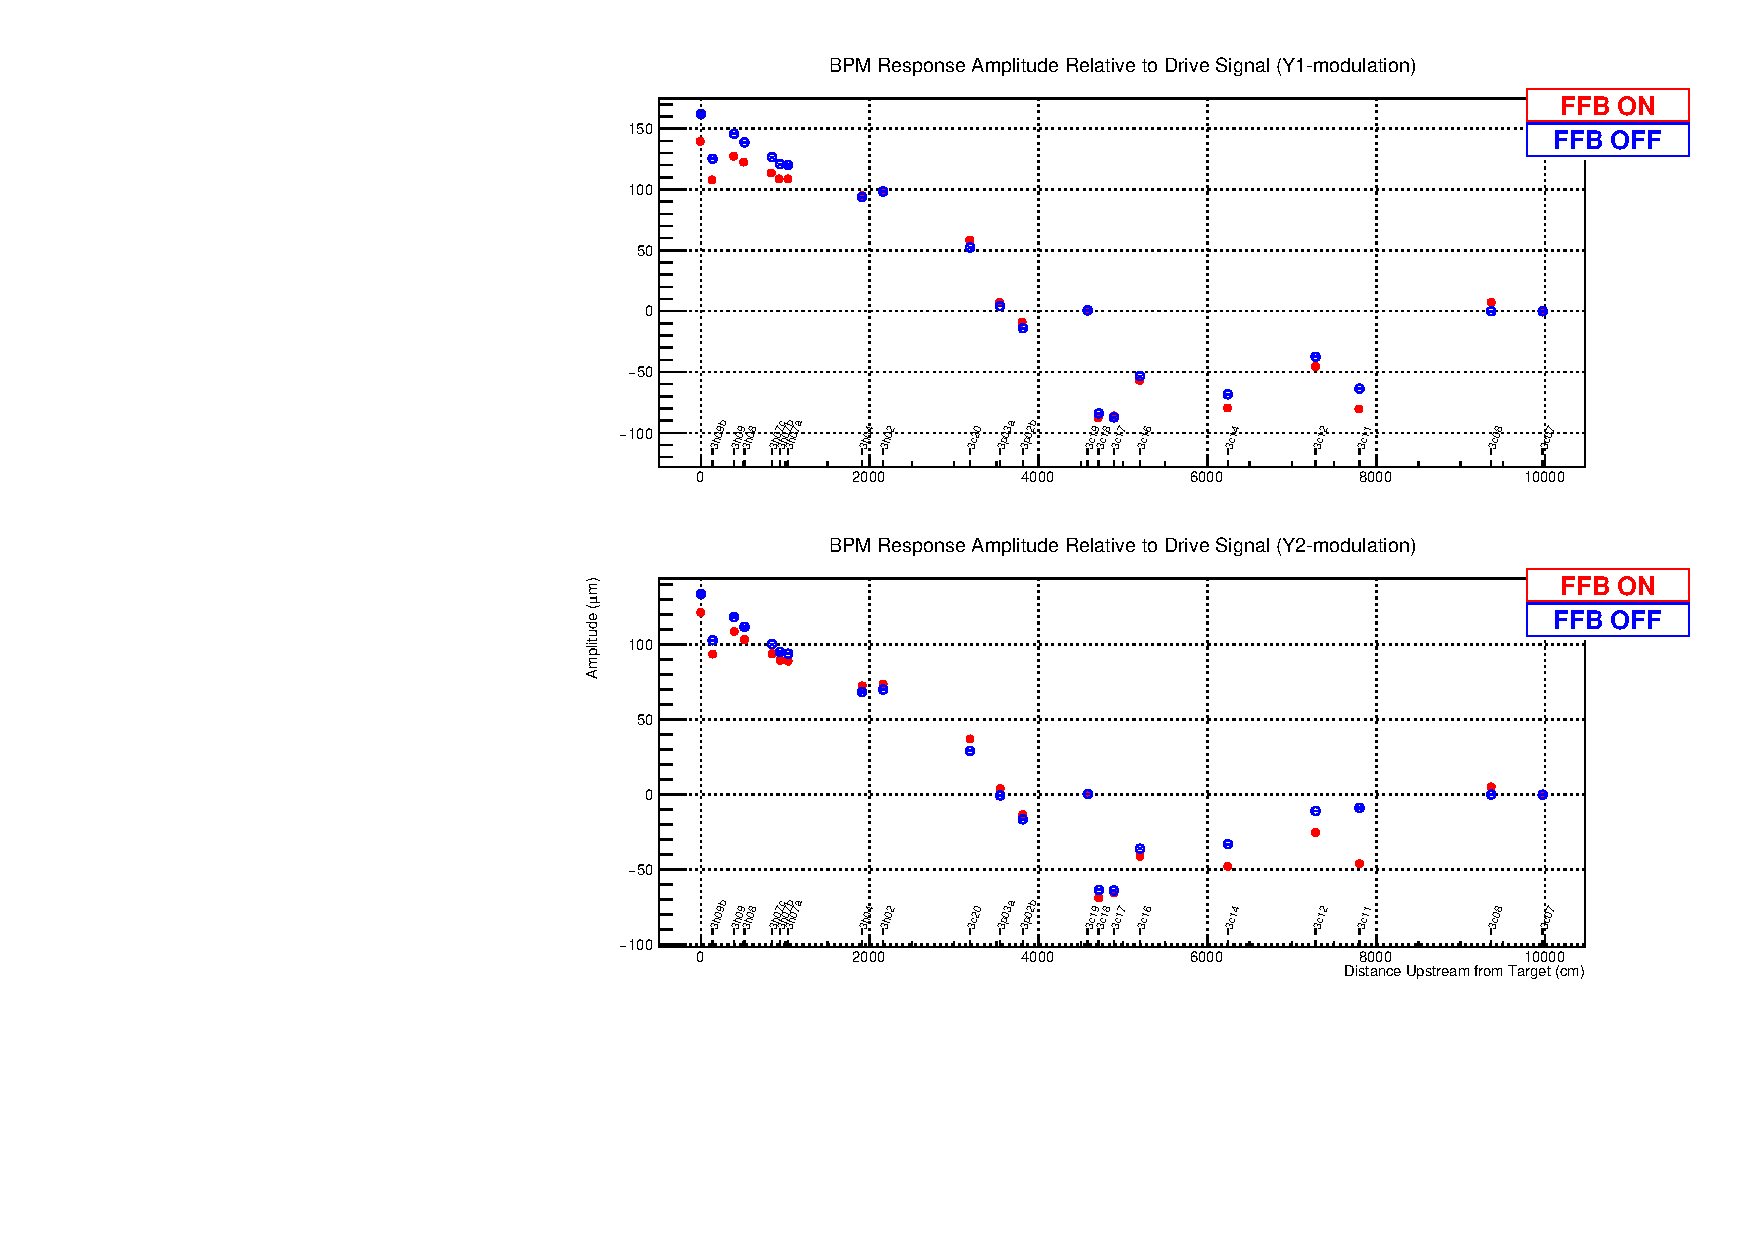
\includegraphics[width=5.6in]{Pictures/bpm_amplitude_vs_z_ymod.pdf}}
\caption{Amplitude of BPM response as a function of distance along beamline upstream from the target. Shown is Y-response to two types of vertical modulation. Notice the relatively small difference between FFB on and FFB off.  This data corresponds to $A(z,\phi)$ in Equation \ref{eq:z_dep_response}. The data for FFB off came from 18445 and for FFB on from 17445 taken about 3 weeks apart.}
\label{fig:bpm_amplitude_vs_z_ymod}
\end{figure}

The effect of FFB on the beam modulation analysis was not understood at first. Since it is an active feedback system, its response to the beam motion may not necessarily be stable or exactly in phase with the modulation coils. The assumption of the simple modulation model given in Equation \ref{eq:det_to_coil} is that all detector and monitor responses at the modulation frequency and in phase with the modulation drive signal are created by actual beam trajectory and energy changes driven by the modulation coils.  An unknown FFB-driven response that is not stable over the modulation period could compromise the integrity of the analysis.
\begin{figure}[ht]
\begin{center}
\framebox{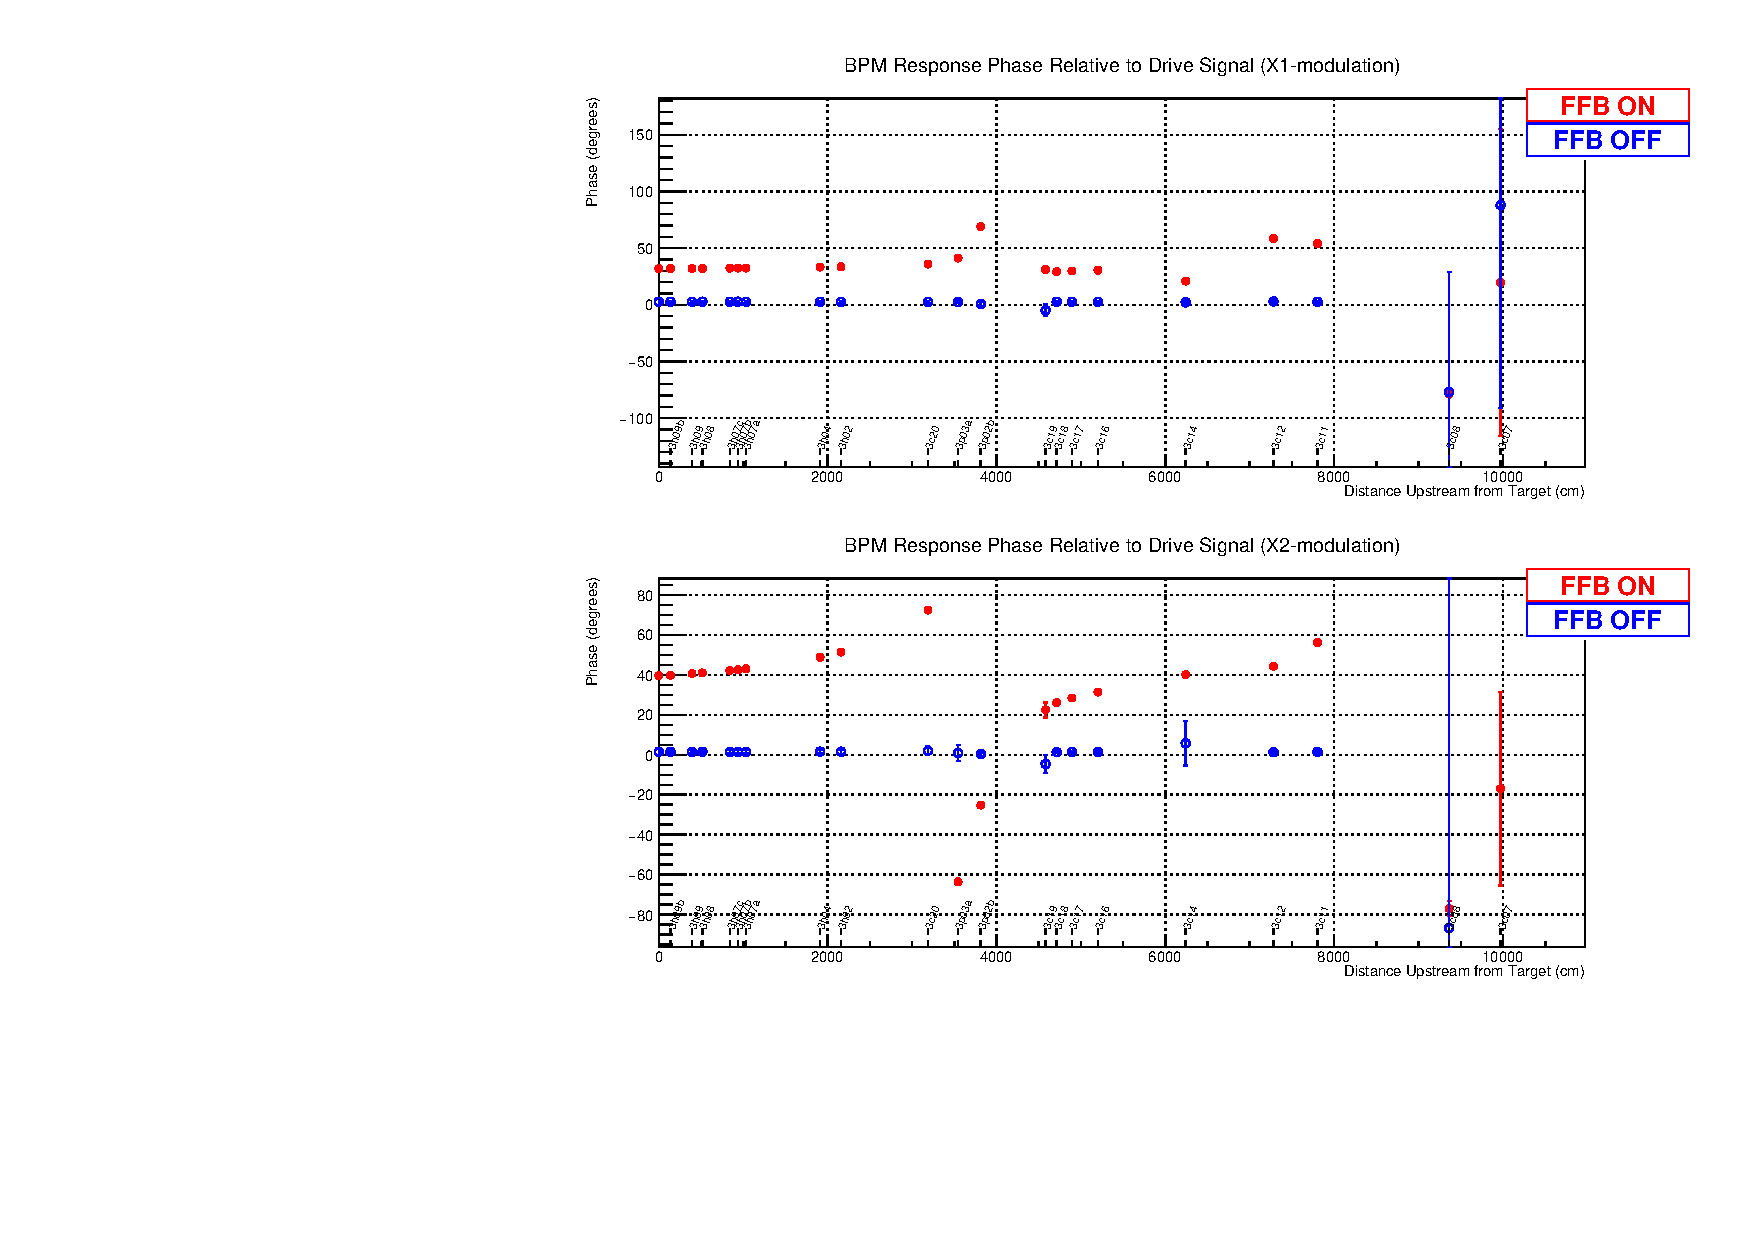
\includegraphics[width=5.6in]{Pictures/bpm_phase_vs_z_xmod.pdf}}
\end{center}
\caption{Phase of BPM response as a function of distance along beamline upstream from the target. Shown is $x$-position response to two types of horizontal modulation. This data corresponds to $\theta (z,\phi)$ in Equation \ref{eq:z_dep_response}.  Notice the phase dependence disappears with FFB off. The data for FFB off came from 18445 and for FFB on from 17445 taken about 3 weeks apart.}
\label{fig:bpm_phase_vs_z_xmod}
\end{figure}
\begin{figure}[ht]
\centering
\framebox{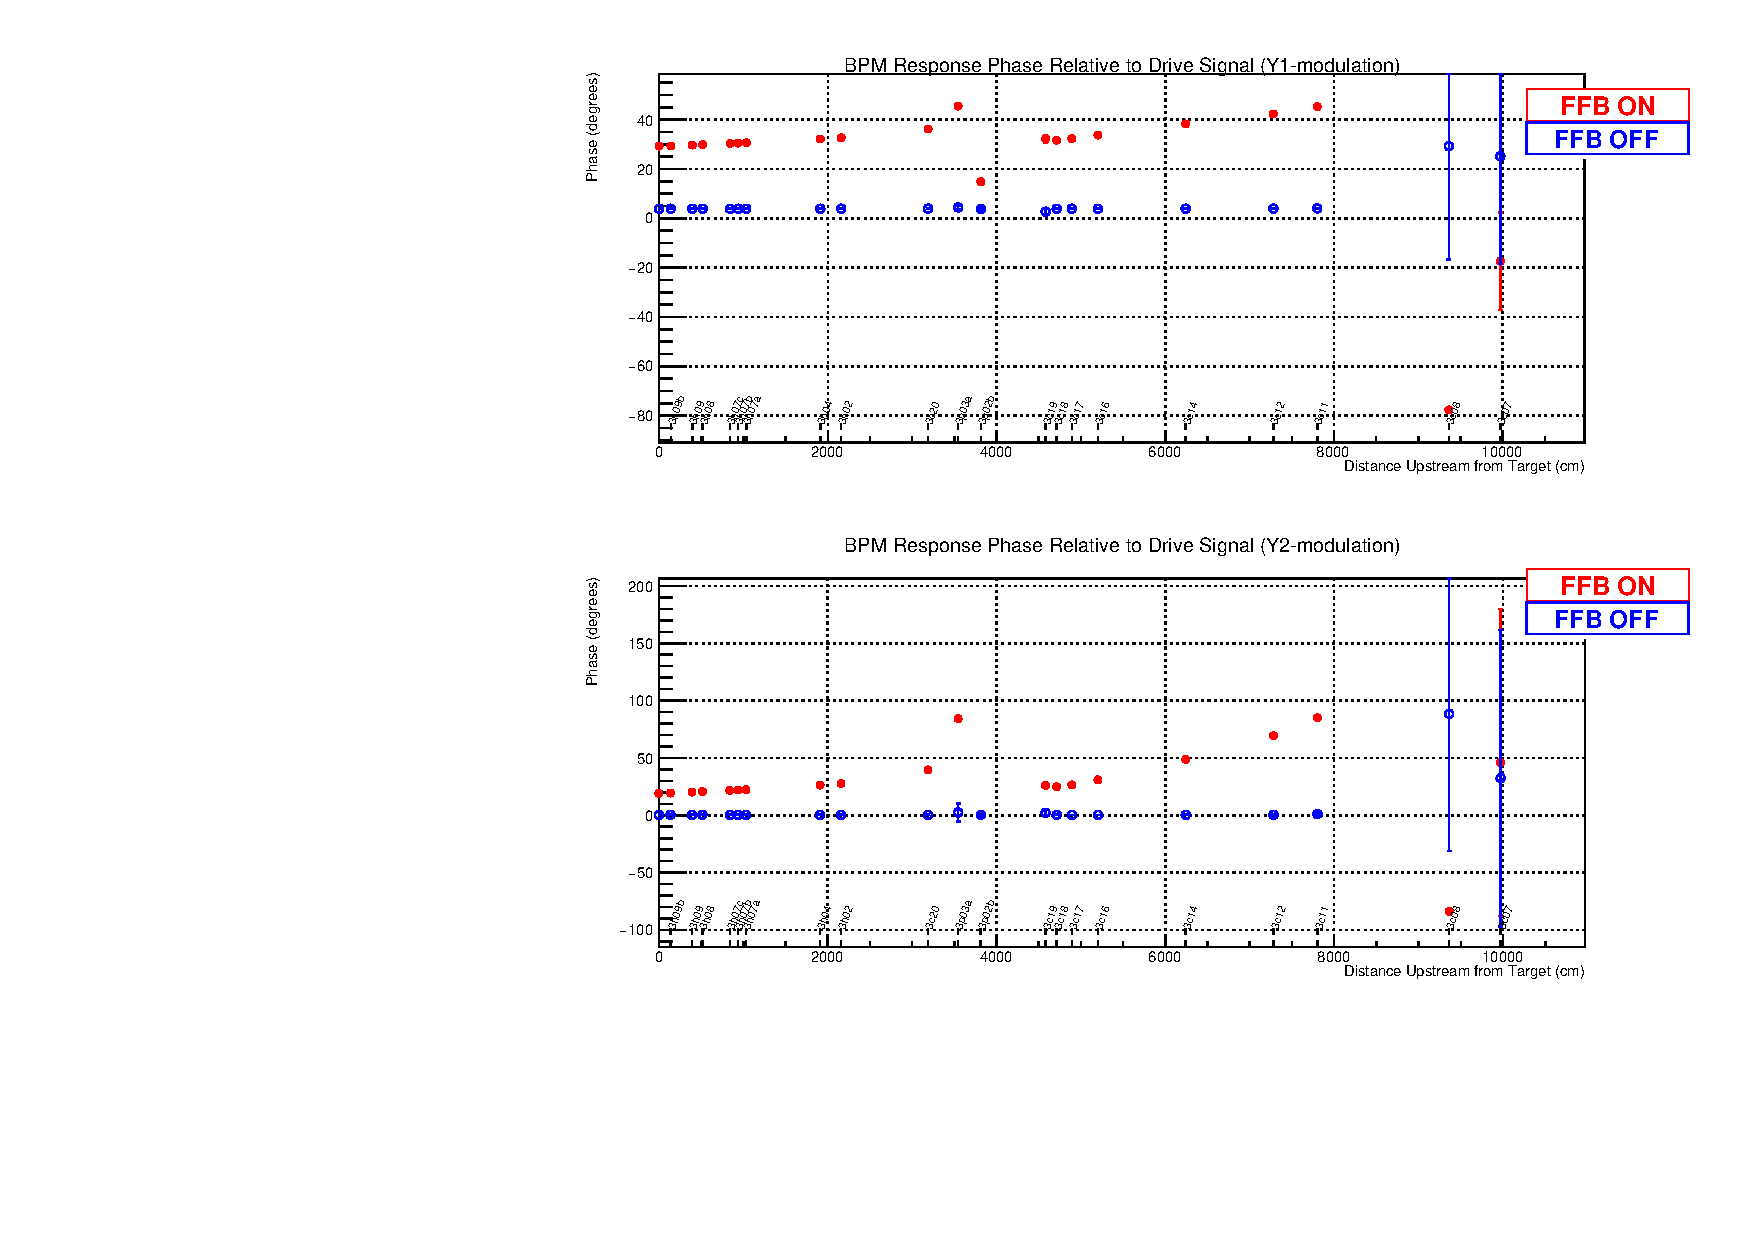
\includegraphics[width=5.6in]{Pictures/bpm_phase_vs_z_ymod.pdf}}
\caption{Phase of BPM response as a function of distance along beamline upstream from the target. Shown is $y$-position response to two types of vertical modulation.  Notice the phase dependence disappears with FFB off.  This data corresponds to $\theta (z,\phi)$ in Equation \ref{eq:z_dep_response}. The data for FFB off came from 18445 and for FFB on from 17445 taken about 3 weeks apart.}
\label{fig:bpm_phase_vs_z_ymod}
\end{figure}

The first indication that the system was not behaving as expected came from a study of BPM responses to beam modulation. The phase of the BPM response relative to the modulation driving signal has an obvious dependence on location along the beamline as seen in Figures \ref{fig:bpm_phase_vs_z_xmod} and \ref{fig:bpm_phase_vs_z_ymod}. This $z$-dependence of the phase can be understood in terms of the optics  of the electron beam. The beam is focused and defocused using quadrupole magnets along the beamline. The beam's size and shape is a function of $z$ (position along the beamline). The relative size and shape of the beam determines the distribution of angle and position trajectories it contains. For example, near a tight focus the electron beam will have a relatively greater spread in electron trajectory angles (measured relative to an ideal reference trajectory) and a relatively small spread in position. Therefore, BPM's positioned near beam focal points will tend to be more sensitive to beam angle shifts and BPM's positioned where the beam spot size changes little with $z$ will be relatively more sensitive to beam position shifts. The phase shifts observed in the BPM responses can be understood in terms of a $z$-dependent response of the electron beam to trajectory changes from the modulation coils, coupled  with a partially out-of-phase FFB response. We can think of a BPM as measuring the in-phase response to the modulation coils plus an out-of-phase response from FFB:
\begin{equation}
\Delta(z,t) = \alpha(z) sin(\omega t) + \beta(z) sin(\omega t + \phi), 
\label{eq:z_dep_response}
\end{equation}
where $\Delta$ is a measured transverse position shift from the ideal beam trajectory, $\alpha(z)$ is the amplitude of the response of the electron beam to the modulation coils at location $z$ along the beamline and $\beta(z)$ is the amplitude of the electron beam response to the FFB coils at z. Using simple trigonometry to recast this equation in terms of a z-dependent phase and amplitude gives
\begin{equation}
\Delta(z,t) = A(z,\phi) sin(\omega t + \theta(z,\phi)), 
\label{eq:z_dependent_phi}
\end{equation} 
where 
\[
A(z,\phi)=\sqrt{\alpha(z)^2+\beta(z)^2+2\alpha(z)\beta(z)\cos(\phi)}
\]
and 
\[
\theta(z,\phi) = tan^{-1}\left( \frac{\beta(z)\sin(\phi)}{\alpha(z)+\beta(z)\cos(\phi)}\right).
\]
In this form, the $z$-dependent phase of the beam response becomes obvious as does its origin in the FFB coil stimulus. Near the end of the \Qs experiment a set of data runs were taken with FFB paused during all modulation periods. The phase of the BPM responses relative to the modulation drive signal can be seen in Figures \ref{fig:bpm_phase_vs_z_xmod} and  \ref{fig:bpm_phase_vs_z_ymod}. The disappearance of the $z$-dependence of the phase when FFB is turned off confirms the hypothesis that it originates from the FFB response.

Having established that the FFB system is responding at the modulation frequency but not in phase with the modulation coils, the next question to address is the stability of this response and the importance of this stability. It is not obvious nor necessary that an active feedback response system will produce a somewhat stable response in time. A more detailed analysis of the stability of the FFB system and its affect on the modulation analysis can be found in Appendix \ref{AppendixB}. At this point it is sufficient to say that the FFB response is not in phase with the drive signal to the modulation coils and that its response is stable enough to be accurately determined over the course of a cycle ($\sim 4~s$). 

As previously mentioned, Equation \ref{eq:chisquaresolution_no_variance} allows for more coils to be used than expected degrees of freedom on the beam. We can make use of as many different linear combinations of the 5 expected degrees as we choose to measure. In this case, with FFB on we have access to the 5 modulation responses in phase with our driving coils and 4 orthogonal $\pi/2$ out-of-phase responses to the FFB coils.\footnote{To be clear, a single sinusoidal response is observed in the monitors and detectors, but it is not in phase with the modulation drive signal. The phase lag is interpreted as the net response to the modulation coils plus a slightly delayed response from FFB coils due to millisecond-scale time constants inherent in the FFB system. The result is a simultaneous driving of two independent modulation modes which can be temporally separated by finding sine and cosine amplitudes.} Of course, this is a simplification since the FFB coils need not be exactly out-of-phase, but we can expect that any out of phase component comes solely from FFB. We only have access to 4 true out-of-phase responses since FFB was paused during energy modulation. A full ``10-Coil'' analysis was performed using the solution of in Equation \ref{eq:chisquare_matrix} where we found 5 in phase and 5 out-of-phase responses which we called ``sine'' and ``cosine'' respectively. Using a full 10 coils instead of the 9 we really have, allows for a potential phase offset between the signal driving the coils and the ``ramp'' signal we fed to our data acquisition electronics to keep track of modulation phase.  

Figures \ref{fig:10Coil_bmod_X_slopes} to \ref{fig:10Coil_bmod_E_slopes} compare the dithering correction slopes found using all 10 coils (Equation \ref{eq:chisquaresolution_no_variance}) and using only the 5 coils in phase with the modulation drive signal (eq. \ref{eq:chisquaresolution_no_variance}). Practically speaking, a 5-Coil ``sine only'' analysis means filling matrix and vector components in Equation \ref{eq:chisquaresolution_no_variance} using only the sine coefficients of the monitor and detector versus modulation phase fits. A 10-Coil analysis uses both the sine and cosine coefficients from the sinusoidal response. A quick comparison shows that these slopes differ greatly from the regression slopes using the same monitors. Perhaps this is not surprising given that the regression slopes minimize the collective noise of the detector by zeroing the detector to monitor correlation, while the slopes for dithering minimize the collective correlation to the coils (drive signals). This does not necessarily mean that dithering zeroes the correlation to coils.

Perhaps more troubling than the difference between regression and dithering slopes is the obvious systematic differences between the two dithering analyses. A few important observations must be made with respect to these differences:
\begin{itemize}
\item{As expected, the 10-Coil analysis with much more information and analyzed using least squares has much smaller error bars than the slopes found with the simple 5-Coil analysis.}
\item{There are large sections of data (see slugs 160-170 for example) where there is not enough information in the ``sine only'' analysis to create useful slopes. The in-phase monitor responses do not sufficiently span the space of beam distortions. However, with the extra information gleaned from the cosine terms, a clean solution for the slopes emerges.}
\item{Rather large inconsistencies in the solutions provided by the two analyses are evidence of an underlying problem in the data or in the analysis procedure. Although correlations and strength sharing between monitors play a role in the slopes ``chosen'' in a regression analysis, they are not expected to influence the dithering analysis very much if at all. The coils simply sample the phase space of possible beam trajectories to allow for measurement of accurate monitor responses. If the monitor responses are stable, the correction slopes found using any complete set of coils is expected to be consistent. A possible caveat to this statement arises if the coils modulate a beam property beyond the 5 in the model and to which the detectors are sensitive.}   
\item{Near the end of the Qweak dataset (after slug 306) the FFB system was paused for all types of modulation. After this, the analysis is reduced to 5 coils since there is little to no out-of-phase response. Because the coils do not sufficiently span the space of beam distortion modes during this period, dithering analysis fails to produce stable correction slopes.}
\end{itemize}

Different slopes do not necessarily mean different total corrections. In a 5-D space with non-orthogonal monitors, there can be many sets of slopes which yield the same total correction. Furthermore, cancellations over time may produce results that appear to be consistent. Table~\ref{tab:dithering_corrections_table} compares the total corrections for MDallbars prescribed by a dithering analyses using all 10 coils and using a 5-Coil ``sine only'' analysis. All corrections are averaged over a Wien states and weighted by the reciprocal of the variance of MDallbars.
\begin{table}[!h]
%table made by ~/thesis_plot_macros/regression_corrections_table.C
\caption{MDallbars dithering corrections compared for analyses with 10 coils and 5 coils (sine only) shown averaged over Wien states. All corrections are weighted by the reciprocal of the square of the main detector error. {\it Note: this table is for purposes of comparison of various regression schemes and does not contain the actual correction and asymmetry values used for \Q. It contains only the data for which there are good dithering slopes for all schemes shown.}}
\begin{center}
\begin{tabular}[h]{|l|c|c|c|}\hline
Wien & Raw Asymmetry & 10-Coil &~5-Coil~~\\
~ & (ppb) & (ppb) & (ppb)\\\hline
  1  & -328.5 & -24.5 & -10.9 \\\hline
  2  & -192.7 & +3.5 & +22.6 \\\hline
  3  & -256.6 & -37.8 & -30.2 \\\hline
  4  & -269.9 & -11.2 & -10.0 \\\hline
  5  & -190.2 & -17.5 & -16.6 \\\hline
  6  & -206.9 & -25.5 & -25.0 \\\hline
  7  & -153.6 & +56.3 & +51.7 \\\hline
  8a & -185.3 & -12.3 & -8.4 \\\hline
  8b & -156.8 & -4.2 & -5.0 \\\hline
  9a & -136.6 & +2.0 & +2.1 \\\hline
  9b & -157.7 & +1.3 & +1.2 \\\hline
  10 & -215.0 & -15.6 & -17.0 \\\hline
\end{tabular}
\end{center}
\label{tab:dithering_corrections_table}
\end{table}

Due to the length and complexity of the topic, the following chapter is devoted entirely to dealing with internal inconsistencies in the dithering dataset.

\begin{figure}[t]
\centering
\framebox{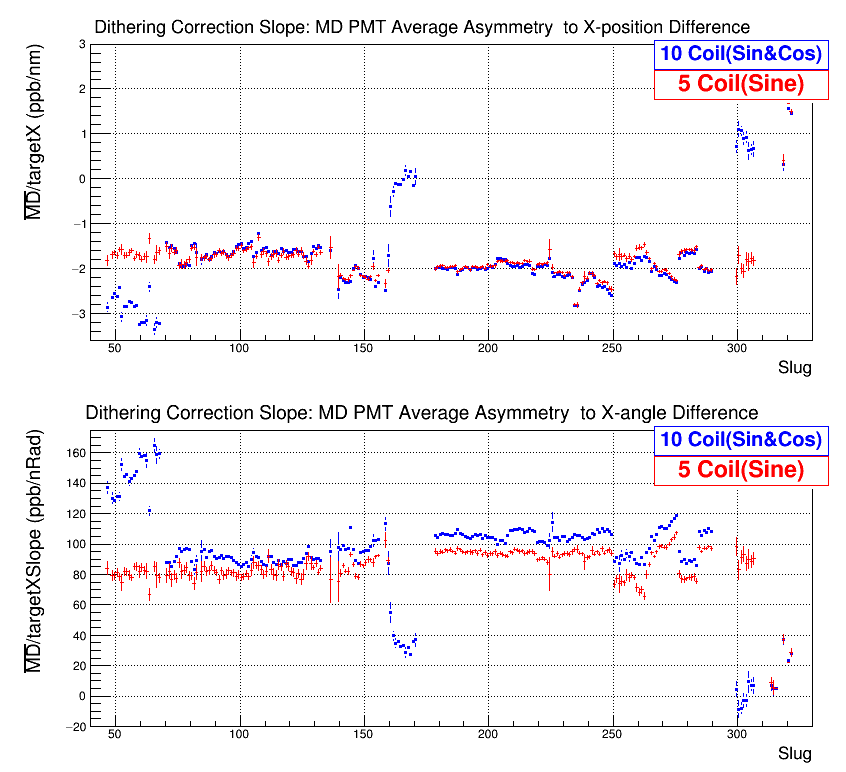
\includegraphics[width=5.5in]{Pictures/10Coil_bmod_X_correction_slopes.png}}
\caption{Dithering correction slopes for horizontal position and angle on target averaged over slugs ($\sim 8~hrs$) using all 10 coils.}
\label{fig:10Coil_bmod_X_slopes}
\end{figure}
\begin{figure}[ht]
\centering
\framebox{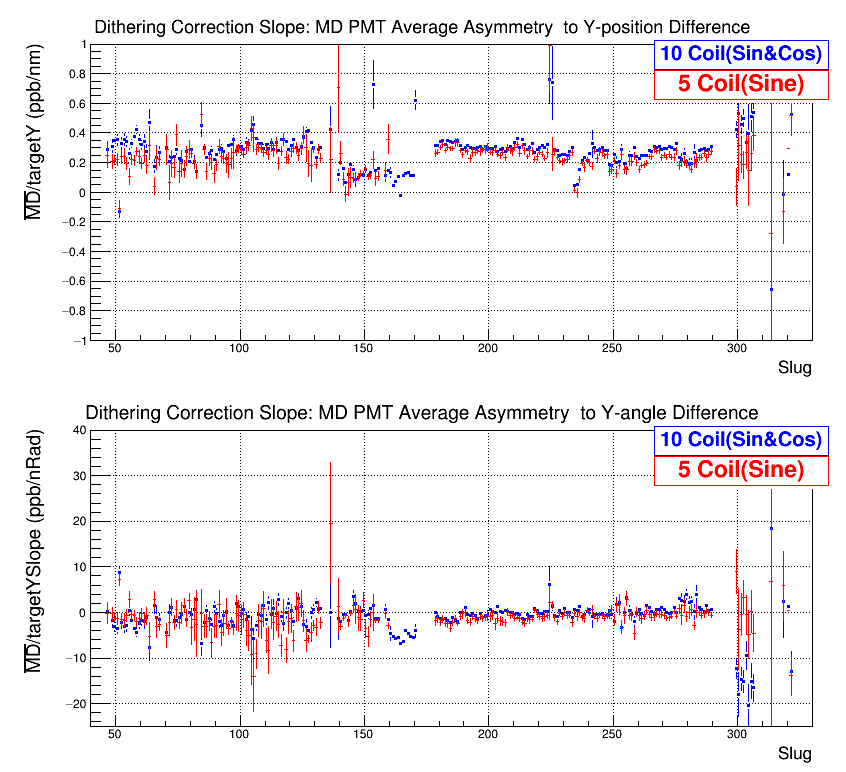
\includegraphics[width=5.5in]{Pictures/10Coil_bmod_Y_correction_slopes.png}}
\caption{Dithering correction slopes for vertical position and angle on target averaged over slugs using all 10 coils.}
\label{fig:10Coil_bmod_Y_slopes}
\end{figure}
\begin{figure}[h]
\centering
\framebox{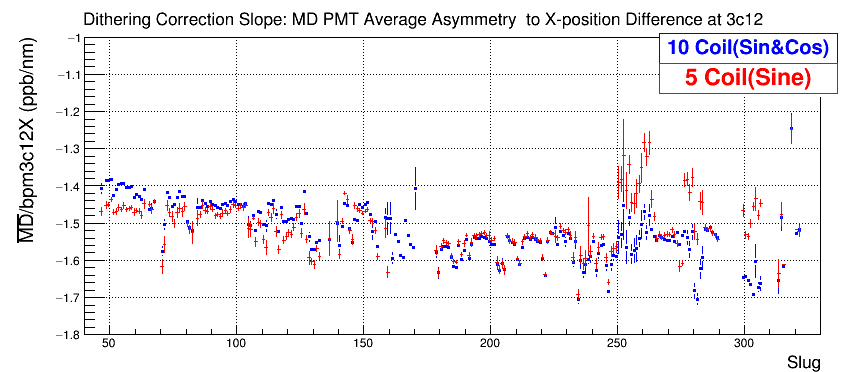
\includegraphics[width=5.5in]{Pictures/10Coil_bmod_E_correction_slopes.png}}
\caption{Dithering correction slopes for horizontal position at bpm3c12 averaged over slugs ($\sim 8~hrs$) using all 10 coils. This is the most energy sensitive monitor on the beamline.}
\label{fig:10Coil_bmod_E_slopes}
\end{figure}

